\documentclass[a4paper]{article}
\usepackage{graphicx}
\usepackage{amsmath, amsfonts, geometry, float, listings, enumerate, multicol}
\usepackage{multicol, float, color, colortbl}
\usepackage{tikz, titlesec, parskip}

\titlespacing{\section}{0pt}{10pt}{0pt}
\titlespacing{\subsection}{0pt}{10pt}{0pt}
\titlespacing{\subsubsection}{0pt}{10pt}{0pt}

\usetikzlibrary{calc,patterns,through}
\newcommand{\arcangle}{%
	\mathord{<\mspace{-9mu}\mathrel{)}\mspace{2mu}}%
}

\renewcommand{\baselinestretch}{1.2}
 \geometry{
 a4paper,
 total={170mm,257mm},
 left=20mm,
 top=20mm,
 }
\usepackage{fancyhdr}
\pagestyle{fancy}
\fancyhf{}
\rhead{\textbf{مقدمه‌ای بر یادگیری ماشین}}
\lhead{\textbf{تمرین سری دوم}}
\cfoot{(\space \space \space \space \textbf{\thepage}  \space \space \space)}
\renewcommand{\headrulewidth}{1pt}
\renewcommand{\footrulewidth}{1pt}
 
\usepackage{xepersian}
%\setlatintextfont{Times New Roman}
\settextfont{XB Niloofar}
\setdigitfont{XB Niloofar}
\DefaultMathsDigits
\usepackage{amsmath}
\usepackage{pgfplots}
\tikzset{declare function={unitstep(\x)=notless(\x,0);}}
\tikzset{declare function={delta(\x)=equal(\x,0);}}

\begin{document}
\begin{minipage}{0.6\textwidth}

\begin{center}
	\begin{bf}
	باسمه تعالی\\
	\vspace{0.25cm}
	دانشگاه صنعتی شریف\\
	\vspace{0.25cm}
	دانشکده مهندسی برق\\
	\vspace{0.5cm}

\large
مقدمه‌ای بر یادگیری ماشین -دکتر جمال‌الدین گلستانی\\
\vspace{0.3cm}
\normalsize
بهراد منیری - ۹۵۱۰۹۵۶۴\\
\Large
\vspace{0.3cm}
گزارش بخش کامپیوتری تمرین سری دوم\\
\vspace{0.4cm}
\end{bf}
\end{center}
\normalsize
\end{minipage} \hfill
\begin{minipage}{0.35\textwidth}

\begin{flushleft}

\includegraphics[width=0.6\textwidth]{Shariflogo.png}\\ \large
\end{flushleft}
\end{minipage}

\section{پیاده‌سازی پرسپترون}
ابتدا الگوریتم پرسپترون را پیاده‌سازی می‌کنیم. کد این الگوریتم در فایل 
\lr{perceptron.m}
نوشته‌شده است. برای بررسی صحت عملکرد این الگوریتم، از داده‌ی مصنوعی دو بعدی برای تست عملکرد آن استفاده کرده‌ام. شکل زیر نمونه‌ای از عملکرد صحیح پیاده‌سازی من از الگوریتم پرسپترون برای داده‌های
\lr{Linearly Separable}
است.

\begin{figure}[h!]
\centering
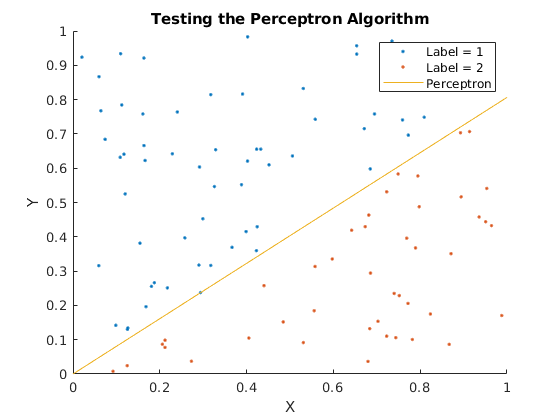
\includegraphics[scale=0.5]{perc.png}
\caption{داده‌های مصنوعی برای تایید صحت عملکرد الگوریتم پرسپترون}
\end{figure}
به نظر می‌رسد که الگوریتم عملکرد درستی دارد.
\section{پرستپترون خطی برای داده‌های ارائه‌شده}
نمودار پراکنش داده‌های ارائه شده به شکل زیر است:
\begin{figure}[h!]
	\centering
	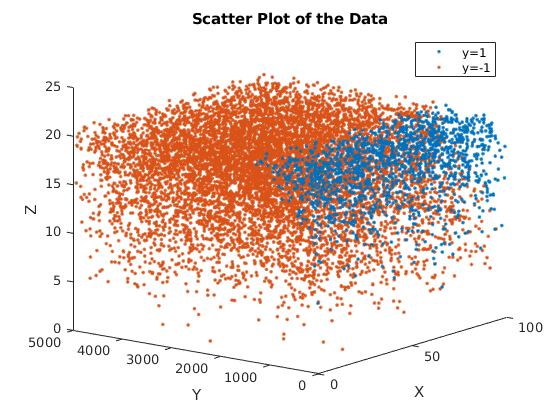
\includegraphics[scale=0.5]{scatter.png}
	\caption{نمودار پراکنش داده‌های ارائه‌شده}
\end{figure}



 تلاش می‌کنیم که به کمک الگوریتم پرسپترون نوشته‌شده در بخش قبل، داده‌های ارائه‌شده را جدا کنیم. 
 
 نمودار زیر، 
 \lr{Loss}
 بر روی داده‌های تست  بر حسب تعداد تکرار در الگوریتم پرسپترون است.
 
 \begin{figure}[h!]
 	\centering
 	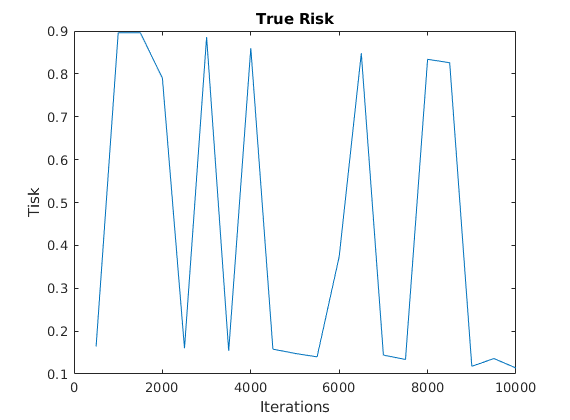
\includegraphics[scale=0.5]{linperc.png}
 	\caption{Loss
 	پرسپترون خطی
 }
 \end{figure}

همچنین بعد از ۱۰۰۰۰ تکرار،
$ \omega = [-0.2458,
-0.0161,
0.9677,
0.0540]$
\section{پرسپترون مکعبی}
 با اضافه کردن توان سوم درایه‌ی سوم، صحت طبقه‌بندی پرسپترون به شدت بهبود می‌یابد. نمودار زیر، تلف پرسپترون است به  ازای تعداد تکرارهای مختلف:
 
 
 \begin{figure}[h!]
 	\centering
 	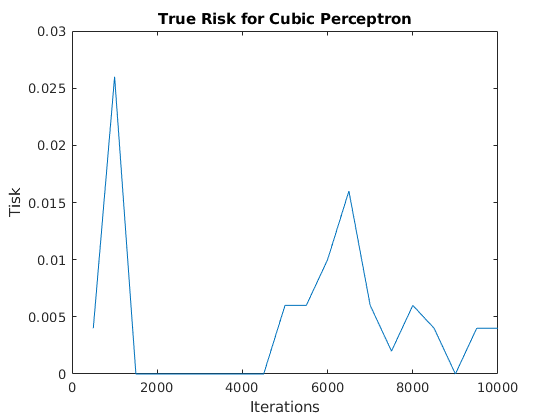
\includegraphics[scale=0.5]{cube.png}
 	\caption{Loss
 		پرسپترون مکعبی
 	}
 \end{figure}
دیده‌ می‌شود که در هر اجرا، به ازای هر تعداد تکرار، حداکثر دو نقطه از ۵۰۰ نقطه اشتباه طبقه‌بندی می‌شوند.
همچنین بعد از ۱۰۰۰۰ تکرار،
$ \omega = [
-0.2198,
-0.9623,
-0.0168,
0.1590,
-0.0013]$
\section{
\lr{SVM}
خطی
}
 با استفاده از تابع 
\lr{fitcecoc}،
\lr{SVM}
را آموزش می‌دهیم. در این حالت خطی، مقدار تلف روی داده‌های تست، برابر 
$0.0140$
و بر روی داده‌های آموزشی، برابر 
$0.0120$
است. بردار 
$\omega$،
در این حالت، برابر است با
$\omega = [
0.0124,
-0.0099,
1.1455]$.


\section{
	\lr{SVM}
مکعبی
}
در این حالت، مقدار تلف بر روی داده‌های تست و آموزشی، برابر صفر است و 
$\omega =
[-0.0104,
-0.2669,
-0.0241,
0.0431]
$.

\section{مقایسه}
با مقایسه‌ی نتایج بخش‌های قبل، به نظر می‌رسد که داده‌‌، ذات درجه سوم داشته و بخش‌های که از مکعب ستون سوم استفاده‌ می‌کنند، نتایج بسیار خوبی می‌دهند. در حالت خطی نیز، روش 
 \lr{SVM}
 به دلیل بیشینه‌کردن مارجین، نتیجه‌ی بهتری از پرسپترون می‌دهد، توجه کنید که داده‌ها به صورت خطی قابل جدا‌سازی نیستند.
\end{document}